%%%%%%%%%%%%%%%%%%%%%%%%%%%%%%%%%%%%%%%%%%%%%%%%%%%%%%%%%%%%%%%%%%%%%%%%%%closed-loop%%%%%%%%%%%%%%%%%%%%%%%%%
\documentclass[letterpaper, 10 pt, conference]{ieeeconf}  % Comment this line out if you need a4paper
                                                          
	%\documentclass[a4paper, 10pt, conference]{ieeeconf}      % Use this line for a4 paper
	%\columnwidth
	\IEEEoverridecommandlockouts                              % This command is only needed if 
															  % you want to use the \thanks command
															  
	\overrideIEEEmargins                                      % Needed to meet printer requirements.  
%	
% See the \addtolength command later in the file to balance the column lengths
% on the last page of the document
%\usepackage[T1]{fontenc}
%\usepackage[latin1]{inputenc}
%
%%%%%%%%%%%%%%%%%%%%%%%%%%%%%%%%%%%%%%%%%%%%%%%%%%%
\usepackage{graphics} % for pdf, bitmapped graphics files
\usepackage{epsfig} % for postscript graphics files
\usepackage{mathptmx} % assumes new font selection scheme installed
\usepackage{times} % assumes new font selection scheme installed
\usepackage{amsmath} % assumes amsmath package installed
\usepackage{amssymb}  % assumes amsmath package installed
%%%%%%%%%%%%%%%%%%%%%%%%%%%%%%%%%%%%%%%%%%%%%%%%%%%
%\usepackage{lmodern}
\usepackage{graphics} % for pdf, bitmapped graphics files
\usepackage{graphicx}     % 
\usepackage{color}
\usepackage{xcolor}
\usepackage{epsfig} % for postscript graphics files
\usepackage{epstopdf}     % conversion to .pdf
\usepackage{url}
\usepackage{calc}
\usepackage{float}
\usepackage{siunitx}
\usepackage{xspace}
\usepackage{standalone}
\usepackage{comment}
\let\proof\relax 
\let\endproof\relax 
\usepackage{amsthm}
\let\labelindent\relax
\usepackage{enumitem}
%%%%%%%%%%%%%%%%%%%%%%%%%%%%%%%%%%%%%%%%%%%%%%%%%%%
\usepackage{tikz}
\usetikzlibrary{positioning,arrows}
%%%%%%%%%%%%%%%%%%%%%%%%%%%%%%%%%%%%%%%%%%%%%%%%%%%

%%%%%%%%%%%%%%%%%%%%%%%%%%%%%%%%%%%%%%%%%%%%%%%%%%%
\usepackage{cite}
\bibliographystyle{IEEEtran}
%
\usepackage{hyperref}
\hypersetup{plainpages = {false},
			bookmarksopen = {true},
			bookmarksnumbered = {true},
			breaklinks = {true},
			pdfstartview={FitH},
			pdfcreator={PDFtime-varyingLaTeX-DPD},	
			pdfproducer={PDFLaTeX-DPD},	
			colorlinks=true,
			citecolor=black,
			linkcolor=black,
			urlcolor=black,
			filecolor=black,
			bookmarksopen=true
} % links em preto
%%%%%%%%%%%%%%%%%%%%%%%%%%%%%%%%%%%%%%%%%%%%%%%%%%%
% Graphical path
\graphicspath{{./Figs/}}
%%%%%%%%%%%%%%%%%%%%%%%%%%%%%%%%%%%%%%%%%%%%%%%%%%%
% TIKZ % ---
% Defining string as labels of certain blocks.
\newcommand{\suma}{\Large$+$}
\newcommand{\sumb}{\Large$\Sigma$}
\newcommand{\minusa}{\Large$-$}
\newcommand{\timesa}{\Large$\times$}
\newcommand{\inte}{$\displaystyle \int$}
\newcommand{\derv}{\huge$\frac{d}{dt}$}

\newcommand{\dd}[1]{ %Marca uma revis�o
    {\color{red}[\![} {\color{blue}\bf#1\xspace} {\color{red}]\!]}
}
\def\re{{\rm I}\! {\rm R}}
\newcommand{\mref}[1]{(\ref{#1})}
\newcommand{\sat}[1]{\mbox{sat}\,}
\renewcommand{\t}{^{\mbox{\tiny\sf T}}} % transposto 
\newcommand\norm[1]{\ensuremath{\lVert#1\rVert}}
\newcommand\abs[1]{\ensuremath{\lvert#1\rvert}}
\newcommand{\matx}[1]{{\textbf #1}}
\def\QED{\mbox{\rule[0pt]{1.0ex}{1.0ex}}} 
\def\proof{\noindent\hspace{2em}{\it Proof: }}
\def\endproof{\hspace*{\fill}~\QED\par\endtrivlist\unskip}
%
\newcommand{\rd}[1]{\textcolor{red}{#1}}
\newcommand{\unit}[1]{\si{#1}}
\newcommand{\myunit}[2]{\num{#1}\,\si{#2}}
%----------------------------------------------------
%  Cross references
%----------------------------------------------------
\newcommand{\tabref}[1]{Tabela~\ref{#1}}
\renewcommand{\eqref}[1]{Eq.~(\ref{#1})}
\newcommand{\figref}[1]{Fig.~\ref{#1}}
\newcommand{\figuref}[1]{Figure~\ref{#1}}
\newcommand\scalemath[2]{\scalebox{#1}{\mbox{\ensuremath{\displaystyle #2}}}}
\setlength{\abovecaptionskip}{0pt}
\setlength{\belowcaptionskip}{-10pt} % reduce space
%%%%%%%%%%%%%%%%%%%%%%%%%%%%%%%%%%%%%%%%%%%%%%%%%%%
%
\theoremstyle{plain}
\newtheorem{theorem}{Theorem}
\newtheorem{lemma}[theorem]{Lemma}
\newtheorem{prop}[theorem]{Proposition}
\newtheorem*{cor}{Corollary}
%
\theoremstyle{definition}
\newtheorem{defn}{Definition}
\newtheorem{conj}{Conjecture}
\newtheorem{exmp}{Example}
%
\theoremstyle{remark}
\newtheorem*{remark}{Remark}
\newtheorem*{note}{Note}
%%%%%%%%%%%%%%%%%%%%%%%%%%%%%%%%%%%%%%%%%%%%%%%%%%%
%
\title{\LARGE \bf
Prosthetic Legs Output Feedback Control via Variable High Gain Observer}


\author{Alessandro J. Peixoto, %
        Ign\'{a}cio de A. M. Ricart and
        Matheus Ferreira dos Reis %and
		%Diego Pereira Dias%		 <-this % stops a space
		%
% <-this % stops a space
}

%%
%%%%%%%%%%%%%%%%%%%%%%%%%%%%%%%%%%%%%%%%%%%%%%%%%%%%%
\begin{document}
%\onecolumn

%%%%%%%%%%%%%%%%%%%%%%%%%%%%%%%%%%%%%%%%%%%%%%%%%%%%%
\DeclareGraphicsExtensions{.pdf,.png,.jpg,.jpeg,.mps,.ps,.eps}
\maketitle
\thispagestyle{empty}
\pagestyle{empty}
%%%%%%%%%%%%%%%%%%%%%%%%%%%%%%%%%%%%%%%%%%%%%%%%%%%%%
\begin{abstract}%
This paper addresses the state estimation and control of a robot/prosthesis control system with four joints: vertical hip displacement, thigh, knee and ankle angles. The motivation was inspired by several drawbacks regarding the usage of load cells and/or sensors in robots and prosthetic legs to capture gait data, external forces (GRFs) and moments during walking. We propose the implementation of a high gain observer (HGO)  to estimate the  prosthesis joint velocities with a time-varying HGO gain synthesized from measurable signals designed to reduce the amount of noise in the control effort while keeping an acceptable tracking error transient performance. Numerical simulations analyze the robustness of the closed-loop control with respect
to parametric errors and measurement noise.
\end{abstract}
%%%
%=============================================================
% INTRODUCTION
%%%%%%%%%%%%%%%%%%%%%%%%%%%%%%%%%%%%%%%%%%%%%%%%%%%%%%%%%%%%%%%%%%%%%%%%%%%%%%%%
\section{Introduction}

Prostheses are devices that substitute the function of a missing limb either due to amputation or a congenital defect. Amputations could occur due to injuries, circulatory and vascular disease, diabetes, smoking or cancer. This means, a huge number of people that could maintain their activities of daily livings (ADLs) and have the mobility partially/completely restored through improvements in prosthesis technology.

The lower limb amputation could be at the foot, including toes or partial foot, at the ankle (ankle disarticulation), below the knee (transtibial), at the knee (knee disarticulation), above the knee (transfemoral) or at the hip (hip disarticulation). Depending on which residual limb remains, mobility could be restored by using a prosthetic foot or, in a worst case scenario, the combination of prosthetic foot/ankle, shin/pylon, prosthetic knee and a socket interfacing the residual limb with the prosthetic leg. 

During the gait, hip, thigh, knee and ankle move expending the minimum metabolic energy, a behavior that resembles that of passive mechanical systems. This motivates the design of prosthesis with moving parts coupled by springs and dampers. Nevertheless, it is also important to generate net power in prosthetic joints through DC electrical motors, pneumatic or hydraulic actuators \cite{Goldfarb2008} \cite{Bedard2002} so that amputees could also realize tasks such as climbing stairs and walking uphill.

Because of that, passive mechanical systems could be used in prosthetics systems, such as springs and dampers with controlled levels as Endolites ankle products and Otto Empower Ankle. However, being able to generate net power in prosthetic joints through DC electrical motors, pneumatic or hydraulic actuators \cite{Goldfarb2008} \cite{Bedard2002} is important so that amputees could also realize tasks such as climbing stairs and walking uphill.

Commonly, the joints angles in a prosthesis are measured with high-resolution encoders, while contact forces are obtained via strain gauges and load cells. Angular velocities could be acquired through expensive tacometers or via estimation. 

In general, numerical approaches for velocity are implemented via state observers or derivative filters, like lead filter. However,  noise attenuation  is a well known challenge in those cases. In this direction, state estimation via Extended Kalman Filter (EKF), High-gain-observer (HGO) and Sliding Mode Observer (SMO) are promising approaches. These techniques could also be used to estimate the contact forces acting on a prosthetic foot.

In contrast to \cite{Fakoorian2016}, where an EKF is designed to estimate joint position, velocities and ground reaction forces, here an HGO based estimation approach is deployed. Time-varying HGOs have also been used to cope with the effect of measurement noise and to establish the connections with the EKF \cite{AK:07}, \cite{Khalil2009}. 

Output-feedback control strategies using HGOs \cite{OK:97} represent an important design class, in particular, the schemes based on time-varying techniques (HGO with variable gain) \cite{P:01}\cite{KKJ:02} \cite{KKC:03}\cite{LL:05}\cite{AK:07}. In \cite{POH:2011}, \cite{PHCL:2007}, an output-feedback sliding-mode control design have been proposed for arbitrary relative degree uncertain systems, where the class of plants encompasses time-varying minimum phase nonlinear plants, affine in the control, transformable to a normal form and for which a norm state estimator can be implemented. The main objective in \cite{POH:2011} was to use a dynamic observer gain in order to obtain global results without invoking global Lipschitz-like restrictions. 

In the present paper, considering that a robot/prosthesis system has parametric uncertainties and angle measurement is subject to noise, a time-varying HGO design is proposed, similar to \cite{POH:2011}. This variable gain approach is different from most of the existing techniques,
where the HGO gain is updated either solving a Riccati equation \cite{P:01}\cite{P:07}\cite{GAL:06} or via functions based on measurable signals and norm domination techniques \cite{LL:05}, \cite{P:07}, \cite{APA:09} and \cite{POH:2011}.

While estimating in real-time the noise energy presented in the control effort, an adaptation law changes the observer gain to achieve a acceptable trade-off between control signal noise and tracking performance. It is important to note that, although global results are not pursued in this paper, the proposed technique is easily applicable to practical scenarios, given that bounds for the system states are known a priori.

A proportional-integral-derivative (PID) conventional control with feedback linearization is developed in order to make a robotic prosthetic leg follow a desired walking pattern. 

The proposed approach is verified in a simulation environment with a $4$-link robot/prosthesis system (PRRR), with parameters extracted from \cite{Richter2015} and motion limited to the sagittal plane. The human gait used as reference signal is obtained from \cite{Schwartz2008}.

%This paper is organized as follows. In Section \ref{sec:System_model}, the system model is described where some considerations regarding the HGO design are taken into. Section \ref{sec:HGO} presents the HGO structure and the adapting function used in simulation. Section \ref{sec:Numerical_Simulation} shows the control law applied to the plant and results obtained. Finally, Section \ref{sec:Conclusions} presents concluding remarks and future work.

\section{Preliminaries}


The following notations and terminology are used:% in the paper:


%\subsection{Notation and Terminology}

%Let $[0,t_M)$ be the maximal time interval of definition of a
%given (plant or controller) solution of system
%(\ref{eq:planta_state}), where $t_M$ may be finite or infinite.
%For any $t_*\!\in\![0,t_M)$ let $\mathcal{I}\!:=\![t_*,t_M)$.

\begin{itemize}

\item The 2-norm (Euclidean) of a vector $x$ and the corresponding
induced norm of a matrix $A$ are denoted by $|x|$ and $|A|$,
respectively. The symbol $\lambda[A]$ denotes the spectrum of $A$
and $\lambda_m[A]=-\max_i\{Re\{\lambda[A]\}\}$.


\item The ${\mathcal{L}}_{\infty e}$ norm of a signal
$x(t)\!\in\!\re^n$ is defined as
$\|x_{t}\|\!:=\!\sup_{0\!\leq\!\tau\!\leq\!t} |x(\tau)|$.


\item  The symbol  ``$s$'' represents either the
Laplace variable or the differential operator ``$d/dt$'', according
to the context. 

\item As in \cite{IS:96} the output $y$ of a linear time invariant (LTI) system with transfer function
$H(s)$ and input $u$ is given by $y=H(s)u$. Convolution operations $h(t)*u(t)$, with $h(t)$ being the impulse response from $H(s)$, will be eventually written, for simplicity, as $H(s)*u$.


\item Classes of $\mathcal{K}, \mathcal{K}_\infty$ functions are
defined according to \cite[p.~144]{K:02}. ISS, OSS and IOSS mean
Input-State-Stable (or Stability), Output-State-Stable (or
Stability) and Input-Output-State-Stable, respectively
\cite{SW:95}.


\item The symbol $\pi$ denotes class-$\mathcal{KL}$ functions. Eventually, we denote by $\pi (t)$ any exponentially decreasing signal, i.e., a signal satisfying $|\pi(t)| \leq \Pi(t)$, where $\Pi(t):=R e^{-\lambda t}$, $\forall t$, for  some scalars $R,\lambda>0$.
\end{itemize}

%%%%%%%%%%%%%%%%%%%%%%%%%%%%%%%%%%%%%%%%%%%%%%%%%%%%%%%%%%%%%%%%%%%%%%%%%

\section{System Model}
\label{sec:System_model}

The dynamics of the machine/prosthesis system composed by a $4$-link rigid body robot\footnote{A more general framework with a $n$-link rigid body robot can also be considered. However, in order to keep this note close to \cite{Richter2015}, for simplicity, we have set $n=4$.} with prismatic-revolute-revolute-revolute (PRRR) configuration, following the notation in \cite{Richter2015} and \cite{Fakoorian2016}, is given by:
%
\begin{equation}
D(q)\ddot{q} + C(q,\dot{q})\dot{q}+B(q,\dot{q}) + P(\dot{q}) + J_e^T F_e+g(q) = F_a\,,
\label{eq:Dinamica}
\end{equation}
%
where  $q$ represents the vector of joints positions ($q_1$ represents the hip vertical displacement, $q_2$ is the thigh angle, $q_3$ is the knee angle and $q_4$ represents ankle angle), $D(q)$ is the inertia matrix, $C(q,\dot{q})$ is the matrix of Coriolis and centrifugal forces, $B(q,\dot{q})$ is the knee  damper nonlinear matrix, $J_e$ is the kinematic Jacobian relative to the point of application of external forces $F_e$, $g(q)$ is the term of gravitational forces and $F_a$ is the torque/force produced by the actuators. The term  $P(\dot{q})$ explicitly represents the Coulomb friction as in \cite{LeeKhalil2015}. Note that, inertial and frictional effects in the actuators can be included in this model. 

To establish a basis for dynamic model derivations and to verify the leg geometry during simulations, the set of reference frames used for forward kinematics problems are the same as the ones assigned in \cite{Richter2015}. Matrices $D(q)\ddot{q}$, $C(q,\dot{q})$ and $g(q)$ are obtained using the standard Newton-Euler recursive approach with the plant parameters extracted from \cite{Richter2015} and \cite{Fakoorian2016}.

\subsection{A Simplified Model}


In order to illustrate the observer design proposed in this note, consider a simplified version of the machine/prosthesis system (\ref{eq:DinamicaSimp}) where no external forces are considered ($F_e \equiv 0$), the specific leg prosthesis damping matrix is disregarded ($B(q,\dot{q}) \equiv 0$) and the  Coulomb friction is neglected  ($P(\dot{q}) \equiv 0$). In this case, the machine/prosthesis system is described by:
%
\begin{equation}
D(q)\ddot{q} + C(q,\dot{q})\dot{q}+g(q) = F_a\,.
\label{eq:DinamicaSimp}
\end{equation}
%
The system matrices $D(q), C(q,\dot{q})$ and $g(q)$ are supposed to be uncertain, but the corresponding nominal matrices  $D_n(q), C_n(q,\dot{q})$ and $g_n(q)$ are assumed known. In particular, the inertia matrix $D(q)$ which is invertible, since $D(q)=D^T(q)$ is strictly positive defined.

Introducing the variables $x_1:=q \in \re^4$ and $x_2:=\dot{q}\in \re^4$, the model (\ref{eq:DinamicaSimp}) can be rewritten in the state-space form as:
%
\begin{subequations}
	\begin{eqnarray}
		\dot{x}_1&=& x_2\,, \\
		\dot{x}_2 &=& k_p(x,t) \left[u+d(x,t)\right]\,, \quad u:=F_a \in \re^{4 \times 1}\,,\\
		y &=&  x_1\,,
\end{eqnarray}
\end{subequations}
%
or, equivalently, 
%
\begin{subequations}
	\begin{eqnarray}
		\dot{x} &=& A_\rho x +  B_\rho k_p(x,t) [u + d(x,t)]\,, \label{eq:plantSS} \\
		y &=& C_\rho x\,,\label{eq:plantSaida} 
	\end{eqnarray}
\end{subequations}
%
where $x^T= \left [ \begin{array}{cc} x_1 & x_2\end{array} \right ]$ is the state vector, $k_p(x,t)=D(x_1)^{-1} \in \re^{4 \times 4}$, $d(x,t):=-C(x_1,x_2) x_2-g(x_1) \in \re^{4 \times 1}$, $C_\rho=\left[\begin{array}{cc} I_{4 \times 4} & 0_{4 \times 4}\end{array} \right] \in \re^{4 \times 8}$ and the pair $(A_\rho, B_\rho)$ is in Brunovskys canonical controllable form and is given by:
%
$$A_\rho=\left[\begin{array}{cccc} 0_{4 \times 4} & I_{4 \times 4}\\
0_{4 \times 4} & 0_{4 \times 4}\end{array} \right] \in \re^{8 \times 8}\,,$$
%
and
%
$$B_\rho=\left[\begin{array}{cc}  0_{4 \times 4} & I_{4 \times 4} \end{array} \right]^T \in \re^{8 \times 4}\,.$$
%
For each solution of (\ref{eq:plantSS}) there exists a maximal
time interval of definition given by $[0,t_M)$, where $t_M$ may be
finite or infinite. Thus, finite-time escape is not precluded, {\em
a priori}.
%
% 
%\begin{remark}({\bf Nominal Values})
%Nominal terms can be used in the HGO implementation in order to reduce conservatism in the HGO design, see the appendix for more details. 
%\end{remark}





%--------------------------------------------------------------------
\section{High Gain Observer with Variable Gain}
\label{sec:HGO}
%--------------------------------------------------------------------

The HGO \cite{Khalil2008} is given by
%
\begin{equation}
\dot{\hat{x}}=A_\rho \hat{x} +  B_\rho k_p^n u +H_\mu L_o (y-C_\rho
\hat{x})\,,\label{eq:reducedHGO}
\end{equation}
%
where $k_p^n$ is a nominal value of the plant high frequency gain (HFG) $k_p$ and $L_o$ and $H_\mu$ are given by:

%
\begin{subequations}
	\label{eq:defLhgo_and_Hhgo}
	\begin{align}
		L_o &= \left[\begin{array}{cc}  l_1 I_{4 \times 4} & l_2 I_{4 \times 4} \end{array} \right]^T \in \re^{8 \times 4} 
		\\
		H_\mu &:= \mbox{diag}(\mu^{-1}  I_{4 \times 4}, \ \mu^{-2} I_{4 \times 4}) \in \re^{8 \times 8}\,.
	\end{align}
\end{subequations}
%
%%
%\begin{remark}({\bf A Temporary Restriction})
%In order to simplify the  HGO (with variable gain) design, without loss of generality, we assume that $k_p$ is {\em known}, i.e., $k_p^{n}=k_p$. Indeed, this restriction can relaxed following a similar procedure as in \cite{jacoud2011}.
%\end{remark}
%
%
The observer gain $L_o$ is such that $s^{2}+l_1
s+ l_2$ is Hurwitz. In this paper,
instead of using a constant $\mu$, we introduce a {\em variable}
parameter $\mu=\mu(t)\neq\!0, \forall t\in[0,t_M)$, %which allows
%us to obtain {\em global} practical tracking. We propose a time
%varying $\mu$
of the form
%
\begin{equation}
\mu(t):=\frac{\bar{\mu}}{1+
\psi_\mu(\omega(t),t)}\,,\label{eq:def_mu}
\end{equation}
%
where $\psi_\mu$, named \textbf{adapting function}, is a
non-negative function continuous in its
arguments and $\omega(t)$ is an available signal, both to be designed later on. This structure will be used so that $\mu \approx \bar{\mu} \pm \delta$, adaptating to a certain criteria.

The parameter $\bar{\mu}\!>\!0$ is a design constant. For each
system trajectory, $\mu$ is absolutely continuous and
$\mu\!\leq\!\bar{\mu}$. Note that $\mu$ is bounded for $t$ in any
finite sub-interval of $[0,t_M)$. Therefore,
%
\begin{equation}
\mu(t)\in[\underline{\mu},\bar{\mu}]\,, \quad \forall
t\!\in\![t_*,t_M)\,, \label{eq:P3}
\end{equation}
%
for some $t_* \in [0,t_M)$ and
$\underline{\mu}\!\in\!(0,\bar{\mu})$. 



%--------------------------------------------------------------------
\subsection{High Gain Observer Error Dynamics}
%--------------------------------------------------------------------

The transformation \cite{OK:97}
%
\begin{equation}
\zeta:=T_{\mu}\tilde{x}\,, \quad T_\mu:=[\mu^2
H_\mu]^{-1} \in \re^{8 \times 8}\,, \quad \tilde{x}:= x-\hat{x}\,,\label{eq:defT_HGO}
\end{equation}
%
is fundamental to represent the $\tilde{x}$-dynamics in 
convenient coordinates allowing us to show that $\tilde{x}$ is
arbitrarily small, {\em modulo} exponentially decaying term. First,
note that:
%
$$(i) \ T_\mu(A_\rho-H_\mu L_o
C_\rho)T_\mu^{-1}\!=\!\frac{1}{\mu}A_o\,, \quad (ii) \ T_\mu B_\rho\!=\!B_\rho\,, \quad$$ 


$$\mbox{and} \quad
(iii) \ \dot{T}_\mu T_\mu^{-1}\!=\!\frac{\dot{\mu}}{\mu}
\Delta\,,$$
%
where $A_o\!:=\!A_\rho\!-\!L_o C_\rho$ and
$\Delta\!:=\!\mbox{diag}(-I_{4 \times 4}, \ 0_{4 \times 4}) \in \re^{8 \times 8}$.
%
Then, subtracting (\ref{eq:reducedHGO}) from
(\ref{eq:plantSS}) and applying the above
relationships (i),
(ii) and (iii), the dynamics of $\tilde{x}$ 
in the new coordinates $\zeta$ (\ref{eq:defT_HGO}) is given by:
%
\begin{equation}
\mu \dot{\zeta} = [A_o+ \dot{\mu}(t) \Delta] \zeta + B_\rho [\mu
\nu]\,, \label{eq:HGO_error_eta}
\end{equation}
%
where %$\Delta(t)\!:=\!\dot{\mu}(t) A_\delta$ and
%
\begin{equation}
\nu:=(k_p-k_p^n)u+k_p d\,,\label{eq:def_nu}
\end{equation}
%
and
%
\begin{equation}
\dot{\mu}(t)\!=\!-\frac{\mu^2}{\bar{\mu}} \left[\frac{\partial
\psi_\mu}{\partial \omega} \dot{\omega}+\frac{\partial
\psi_\mu}{\partial t}\right]\,. \label{eq:def_mudot}
\end{equation}
%
%Colocar em funcao de $u_{av}$.
The HGO gain ($H_\mu L_o$) is inversely proportional to the small parameter $\mu$,
allowed to be time-varying. % in order to guarantee global tracking. 
Our task is to establish properties for the adapting
function $\psi_\mu(\omega(t),t)$ in (\ref{eq:def_mu}) so that $\mu
|\nu|$ and $|\dot{\mu}|$ are arbitrarily small, at least after a
finite time interval. In fact, we design $\psi_\mu$ so that the following inequalities hold
%
\begin{equation}
|\dot{\mu}(t)|\,, \ \mu |\nu| \leq \mathcal{O}(\bar{\mu})\,, \quad
\forall t \in [t_\mu,t_M)\, \label{eq:mudotmunu}
\end{equation}
%
for  some finite $t_\mu \in [0,t_M)$.  Consequently, $\dot{\mu}$ does not {\em
ultimately} affect the stability of $A_o$ in
(\ref{eq:HGO_error_eta}) and $\zeta$  can be made
arbitrarily small, {\em modulo} an exponentially decaying term, by applying a time scale changing in (\ref{eq:HGO_error_eta}). In addition, since $\tilde{x} = T_\mu^{-1} \zeta$ and $\|T_\mu^{-1}\|$ is of order $\mathcal{O}(1)$, then one can conclude that $\tilde{x}$ can also be made
arbitrarily small, {\em modulo} an exponentially decaying term.

It is clear that inequalities in (\ref{eq:mudotmunu}) depend on the choice of the control signal $u$ in (\ref{eq:def_nu}), the disturbance and the signal $\omega(t)$. 

\subsection{The Adapting Function $\psi_\mu$}

The adapting function $\psi_\mu(\omega(t),t)$ used in the time-varying parameter 
%
\begin{equation}
\mu(t):=\frac{\bar{\mu}}{1+
\psi_\mu(\omega(t),t)}\,,%\label{eq:def_mu}
\end{equation}
%
defined in (\ref{eq:def_mu}), can assume different forms depending on the choice of the signal $\omega(t)$ and the available information about the plant. 

As an example, consider the following cases:
%
\begin{enumerate}

\item {\bf From a theoretical point of view}: the adapting function $\psi_\mu$ can be chosen in order to allow global/semi-global stability (or only convergence) properties for the closed-loop control system. 

\begin{enumerate}

\item {\bf Norm Observability}: The plant
(\ref{eq:plantSS})--(\ref{eq:plantSaida}) admits a norm observer which provides an upper bound for the plant state norm by using only  available signals: plant input ($u$) and plant output ($y$). In this case, global or semi-global results could be obtained when, for example, a sliding mode based control is employed, as in \cite{POH:2011}.  


More precisely, a norm observer for system
(\ref{eq:plantSS})--(\ref{eq:plantSaida})  is a $m$-order
dynamic system of the form:
%
\begin{align}
\tau_1 \dot{\omega}_1 &= -\omega_1+u\,, \label{eq:defuav} \\
%\tau_2 \dot{\omega}_2 &= - \gamma_o(\omega_2) + \tau_2
%\varphi_o(\omega_1,y,t)\,,\label{eq:normobsgeneric}
\tau_2 \dot{\omega}_2 &=
\gamma_o(\omega_2)+\tau_2\varphi_o(\omega_1,y,t)\,,\label{eq:normobsgeneric}
\end{align}
%
with states $\omega_1\!\in\!\re$, $\omega_2\!\in\!\re^{m\!-\!1}$ and
positive constants $\tau_1, \tau_2$ such that for $t\in[0,t_M)$: (i)
if $|\varphi_o|$ is uniformly bounded by a constant $c_o\!>\!0$,
then $|\omega_2|$ can escape at most exponentially and there exists
$\tau_2^*(c_o)$ such that the $\omega_2$-dynamics is BIBS
(Bounded-Input-Bounded-State) stable w.r.t. $\varphi_o$ for
$\tau_2\leq \tau_2^*$; (ii)
for each $x(0),\omega_1(0),\omega_2(0)$, there exists $\bar{\varphi}_o$ such that
%
\begin{equation}
|x(t)| \leq \bar{\varphi}_o(\omega(t),t) + \pi_o(t) \,, \quad
\omega:=[\omega_1 \ \omega_2^T \ y]^T\,,\label{eq:xboundfromw}
\end{equation}
%
where
$\pi_o:=\beta_o(|\omega_1(0)|\!+\!|\omega_2(0)|\!+\!|x(0)|)e^{-\lambda_o
t}$ with some $\beta_o \in \mathcal{K}_\infty$ and positive
constant $\lambda_o$.

\item {\bf Global Stability Properties}: when the class of plants are such that a norm observer can be implemented, then {\bf global} results can be achieved via Output Feedback Sliding Mode (OFSM) control, as in \cite{POH:2011}. This is the case  when, for example, the Coriolis term can be neglected ($C(x_1,x_2) x_2 \equiv 0$).


\item {\bf Semi-Global Stability Properties}:  it is not a restrictive assumption consider the existence of a class $\mathcal{K}_{\infty}$ function $\Psi(\cdot)$ and a positive constant $k_\psi$ such that 
%
$$\|d(x,t)\| \leq \Psi(\|x\|) + k_\psi\,,$$
%
$\forall x$ and $\forall t$. In other words, the disturbance 
can always be norm bounded afinelly in the state norm, when it is norm bounded in the second argument. Thus, given $R>0$ and $0<R_0<R$, then for some $t^* \in (0,t_M)$ and $\|x(0)\| < R_0$ one has $\|x(t)\| < R$ for $t \in [0,t^*)$. Assume $t \in [0,t^*)$. Since the  nonlinear terms in the robot dynamic equation are usually assumed sufficiently smooth and locally Lipschitz in its arguments, then  $\Psi(\cdot)$ can be chosen locally Lipschitz in it argument. In
addition, while $t \in [0,t^*)$, the state $x$ is
bounded by the arbitrary constant $R$. Thus, one has that the following upper bound holds $\Psi(\|x\|) \leq \kappa(R)\|x\|$, where $\kappa(\cdot)$
being of class $\mathcal{K}$. For a given $R$, $\kappa(R)$ is a
positive constant which increases as $R \rightarrow +\infty$, but
is not necessarily unbounded. By noting that $R$ depends on the initial condition (due to $R_0$), then only {\bf semi-global} stability properties follows. In fact, this semi-global result  can be obtained via a particular case of the OFSM control given in \cite{POH:2011}. This is the case  when, for example, the Coriolis term can not be neglected ($C(x_1,x_2) x_2 \neq 0$).

\end{enumerate}


\item {\bf From a practical point of view}: the adapting function $\psi_\mu$ can be chosen in order to allow local stability (or only convergence) properties for the closed-loop control system. Moreover, one can select a time-varying adapting function $\psi_\mu$ to assure an acceptable level of noise in the control signal while keeping a good transient for the output tracking error. 

\begin{enumerate}


\item {\bf The system states can be assumed bounded}: The plant state, in particular the unavailable state $x_2$, is uniformly bounded. Such assumption of the state boundedness is true, for example, when (\ref{eq:plantSS}) is BIBS stable, and the control input is bounded. Moreover, by considering that the acceleration ($\dot{x}_2$) in the mechanical system is bounded by a known constant, then a constant  upper bound for the velocity $x_2$ can be found by using the ``dirty derivative'':
%
\begin{equation}
\eta := \frac{\tau}{\tau s+1} y\,.
\end{equation}
%
Indeed, by noting that 
%
\begin{equation}
x_2=\eta + \frac{\tau}{\tau s+1} \dot{x}_2\,,
\end{equation}
%
one can obtain the following norm bound  
%
\begin{align}
	|x_2| \leq |\eta| + \mathcal{O}(\tau) \, |\dot{x}_2| \, .
\end{align}
%
In this case, we can use this rough estimate for $\dot{x}_2$ and less conservative estimates for the terms depending on $y$, so that $\omega(t)$ can be implemented.


\item {\bf Signal-to-Noise Ratio in $|u|$ \  $\times$ \ Tracking Error Norm}: By using some measurement of the amount of noise in the control signal, for example, the Signal-to-Noise Ratio (SNR), the adapting function can be implemented as a function of the SNR and the tracking error, so that $\mu$ increases when the SNR in the control effort increases and $\mu$ decreases when the tracking error norm increases. This can be accomplished, for example, by defining a cost function depending on the control signal-to-noise ratio and the output tracking error, so that the time-varying $\mu$ reaches an optimum value.
\end{enumerate}

 
\end{enumerate}



%--------------------------------------------------------------------
\subsection{One Particular Design for $\psi_\mu$}
%--------------------------------------------------------------------
%
%When the plant (\ref{eq:plantSS})--(\ref{eq:plantSaida}) admits a norm observer with $\omega$ defined in (\ref{eq:xboundfromw}) such that 
%%
%\begin{equation}
%|x(t)| \leq \bar{\varphi}_o(\omega(t),t) + \pi_o(t)\,,\label{eq:xboundfromw1}
%\end{equation}
%%
%then norm bounds for the signals $\nu, \dot{\omega}$ and $\dot{\mu}$ can be obtained so that \cite{POH:2011}:
%%
%\begin{equation}
%|\dot{\mu}(t)|\,, \ \mu |\nu| \leq \mathcal{O}(\bar{\mu})\,, \quad
%\forall t \in [t_\mu,t_M)\,, \label{eq:mudotmunu1}
%\end{equation}
%%
%where $t_\mu \in [0,t_M)$. In this case, using the OFSM control described in \cite{POH:2011}, global, semi-global or local stability and/or convergence properties can be assured by noting that the output tracking error dynamics (and the full error system dynamics) is ISS w.r.t. HGO estimate error  which can be made of order $\mathcal{O}(\bar{\mu})$ after the small finite time instant $t_\mu$. For more details, see \cite{POH:2011}.
%

In this paper, we are focused in the following particular choice for time varying HGO gain $\mu(t)$ where noise energy in the control signal and tracking error are taken into account: 
%
\begin{equation}
\mu(t):=\frac{\alpha \mathcal{N}\{u\}}{1+\beta |e|}=\frac{\bar{\mu}}{1+
\psi_\mu(\omega(t),t)}\,,\label{eq:def_mupratico}
\end{equation}
%
where $\alpha,\beta$ are positive design constants, $\mathcal{N}\{u\}>0$ is the noise energy presented in the control effort $u(t)$ and $e$ is the tracking error. Note that, this choice fits the general format (\ref{eq:def_mu}) with $\psi_\mu(\omega(t),t)=[(1+\beta |e|) \bar{\mu}-\alpha \mathcal{N}\{u\}]/(\alpha \mathcal{N}\{u\})$ and $\bar{\mu}$ small enough to assure that  $\psi_\mu(\omega(t),t)>0$. 

The noise energy is obtained by filtering the norm of the difference between 
the upper $U^{+}$ and lower $U^{-}$ envelopes of the control signal $u$ which is contaminated by noise. The noise energy $\mathcal{N}\{u\}$ is defined as:
%
%
$$\mathcal{N}\{u(t)\}:=\frac{1}{\tau_n s +1} \left|U^{+}(t)-U^{-}(t)\right|\,,$$
%
where $\tau_n>0$ is a design constant. Several  on-line methodologies for estimation of noise energy in a available signal (Signal-to-Noise Ratio) can be found in the literature. A fair comparison is left for a future work.  


Note that, in this case, the time derivative $\frac{d \mathcal{N}\{u(t)\}}{dt}$ can be norm bounded if the noise energy is norm bounded, which is reasonable to assume. Therefore, one can verify that  (\ref{eq:mudotmunu}) holds following the a similar approach as the one described in \cite{POH:2011}. 


%--------------------------------------------------------------------
\subsection{Norm Bounds for the HGO Estimation Error}
%--------------------------------------------------------------------

The following lemma can be stated.

\begin{lemma}\label{lemma:HGO}
Consider the HGO error dynamics
(\ref{eq:HGO_error_eta}). Then, if the HGO time varying parameter $\mu(t)$  in (\ref{eq:def_mu}) is designed to satisfy (\ref{eq:mudotmunu})  
during the interval $t \in [t_\mu,t_M)$, then the observer
error norm $|\tilde{x}(t)|$ is bounded by a constant of order
$\mathcal{O}(\bar{\mu})$, {\em modulo} an exponentially decaying
term depending on the HGO initial condition.
\end{lemma}
\proof
Consider the $\zeta$-dynamics
(\ref{eq:HGO_error_eta}) and the storage $V=\zeta^T P \zeta$,
where $P=P^T>0$ is the solution of $A_o^T P + P A_o=-I$. Then, the
time derivative of $V$ along the solutions of
(\ref{eq:HGO_error_eta}) satisfies
%
$\mu \dot{V} = - |\zeta|^2 + (\dot{\mu}) [2 \zeta^T P \Delta
\zeta] + (\mu \nu) [2 \zeta^T P B_\rho]$.
%
Now, designing $\mu$ to satisfy (\ref{eq:mudotmunu}), the following inequality is valid $\forall
t \in
[t_\mu,t_M)$:
%
$\mu \dot{V} \leq - |\zeta|^2 + \mathcal{O}(\bar{\mu}) k_1
|\zeta|^2 + \mathcal{O}(\bar{\mu})k_2 |\zeta|$,
%
where $k_1:=2|P||\Delta|$ and $k_2:=2 |P| |B_\rho|$. Moreover,
since $ab < a^2 + b^2$, for any positive real numbers $a,b$, then
%one has
%
$$\mu \dot{V} \leq - [1 - \mathcal{O}(\bar{\mu}) k_1-\mathcal{O}(\bar{\mu}) ] |\zeta|^2
+\mathcal{O}(\bar{\mu})\,,$$
%\mathcal{O}(\bar{\mu})k_2 |\zeta| + \pi_3^2\,,$$
%
from which one can conclude that $\mu \dot{V} \leq -\lambda_1 V +
\mathcal{O}(\bar{\mu})$, with an appropriate constant
$\lambda_1>0$. Now, either
$V\leq2\mathcal{O}(\bar{\mu})/\lambda_1$ or $\mu \dot{V} \leq
-\lambda_1 V/2$. Consider the later case. Since $\mu<\bar{\mu}$,
then one has $\dot{V} \leq -\lambda_1V/(2\bar{\mu})$. Hence, one
can conclude that 
%
$$|\zeta|\,,|\tilde{x}| \leq
\beta_2(|\zeta(0)|) e^{-\lambda_2 t} + \mathcal{O}(\bar{\mu})\,,$$
%
$\forall t \in [t_\mu,t_M)$, with an appropriate constant
$\lambda_2>0$ and some $\beta_2 \in \mathcal{K}_\infty$. In the
last inequality, the norm bound for $\tilde{x}$ was obtained
by reminding that $\tilde{x}\!=\!T_\mu^{-1} \zeta$, by definition, which  implies
$|\tilde{x}| \!\leq\! |\zeta|$, since $|T_\mu^{-1}|\!\leq\!1$
for $\mu\!<\!1$. \endproof

\section{Problem Formulation and Control Schemes Stability Properties}

The {\em control objective} is to reduce the tracking error 
%
\begin{align}
e(t) := & y_{d} - y\,,
\end{align}
%
where the desired trajectory $y_d$ is ideally a set of joint angles acquired for human gait analysis \cite{Schwartz2008}.  A second-order model reference linear filter % with transfer function
%
%\begin{align}
%	H(s) = \frac{w_{n}^2}{s^2 + 2\zeta \omega_n + \omega_n^2}
%\end{align}
%
has been designed so that the reference signal is actually a filtered version of human gait desired angles. This allows us to obtain directly the  time-varying derivatives $\dot{y}_d$ and $\ddot{y}_d$ from the state vector representation of the model reference filter.

In order to focus on the behavior of the HGO with time varying gain, a simple  PID controller with feedforward is employed  in this note. So, only local stability properties are assured in presence of uncertainties in the plant parameters and in the HGO estimates. Global/semi-global stability properties can be obtained by using the  OFSM controller previously developed in \cite{POH:2011}.

By recalling that we  consider $D_n(y)=D(y)$ to simplify the paper presentation, the control  signal is given by
%
\begin{align}
u(t) := & D(y) u_v + C_{n}(y,\hat{x}_2) \hat{x}_2+g_{n}(y)\,, \\
u_v(t):= &\ddot{y}_d + K_p e(t) + \underbrace{K_d (\dot{y}_d - \hat{x}_2)}_{\approx K_d \frac{de(t)}{dt}} + K_i\int_{0}^{t}e \, dt\,,
\label{eq:defu}
\end{align}
%
where $\hat{x}_2$ is the estimate for $x_2$ obtained from the HGO. The gains are designed in order to match the following equations
%
\begin{align}
	s^3 + K_ds^2 + K_ps + K_i &= 0\,, \\
	(s^2 + 2\zeta \omega_n + \omega_n^2)(s + p) &= 0\,,
\end{align}
%
where $\omega_n$, $\zeta$ and $p$ are design constants and $K_i := k_i(I_{4 \times 4})$, $K_p := k_p(I_{4 \times 4})$ and $K_d := k_d(I_{4 \times 4})$. Therefore the controller gains are designed in order to approximate the error third order dynamics to a second order system added to a (fast) pole. To this end, the control gains are designed as:
%
\begin{align}
	k_i &:= \omega_n^2p\,, \\
	k_p &:= \omega_n^2 + 2\zeta \omega_n p\,, \\
	k_d &:= p + 2\zeta \omega_n\,. 
\end{align}
%


\subsection{Stability Properties}

When uncertainties are presented in the plant parameters and in the HGO estimates, one can write:
%
%
\begin{align}
\ddot{e} + K_d \dot{e} + K_p e + K_i\int_{0}^{t}e \, dt = \xi(t)\,,
\label{eq:closed}
\end{align}
%
where 
%
\begin{eqnarray}
\xi(t)&:=&-D^{-1}(y) (C_n(y,\hat{x}_2)-C(y,x_2)) x_2 -  \\  \nonumber
& -& D^{-1}(y)\left[(g_n(y)-g(y))-C_n(y,\hat{x}_2) \tilde{x}_2)\right]-K_d \tilde{x}_2\,.
\end{eqnarray}
%
Note that, in the ideal case when the nominal matrices $C_n$ and $g_n$ match the real values and $\hat{x}_2=x_2$, the following closed-loop equation holds
%
\begin{align}
\dddot{e} + K_d \ddot{e} + K_p \dot{e} + K_i e =0\,,
\label{eq:closed}
\end{align}
%
which assures that $|e(t)| \rightarrow 0$ as $t \rightarrow \infty$ when  $s^3 + K_d s^2 + K_p s + K_i = 0$ has strictly stable roots. 



For the general case, when uncertainties are presented in the plant parameters and in the HGO estimates, the tracking error converges (locally) to a residual set of order $\mathcal{O}(\bar{\mu})$, where $\bar{\mu}$ is the small parameter in the time varying HGO parameter $\mu(t)$. In what follows, the stability analysis is carried out for $k_i=0$ for simplicity. However, the case $k_i \neq 0$ can be treated in a similar fashion. 

First, for $k_i=0$, one has that the closed loop error dynamics becomes 
%
$\ddot{e} + K_d \dot{e} + K_p e  = \xi(t)$
%
which can be made ISS w.r.t. $\xi$ by appropriate values of $K_p,K_d$ so that $s^2 + K_d s + K_p$ is a Hurwitz polynomial. Second, by considering the plant state satisfies $\|x(t)\| < M$, $\forall t<t^*$ and some $t^*>t_\mu$, then by applying Lemma~\ref{lemma:HGO}, the disturbance term norm $\| \xi \|$ is bounded by a constant of order $\mathcal{O}(\bar{\mu})$, {\em modulo} an exponentially decaying term depending on the HGO initial condition. Since the tracking error dynamics is ISS w.r.t. $\xi$, then one can conclude that $e(t)$ ultimately converges to a residual set of order $\mathcal{O}(\bar{\mu})$. This is a local convergence property. 

  
On the other hand, when the OFSM control scheme developed in \cite{POH:2011} is considered,  global/semi-global practical stability results can be guaranteed, even in the presence of those uncertainties. This was left for a future work.


%The formal proof of this stability results were omitted to save space and to focus on the HGO variable gain behaviour. However, we highlight that  the OFSM control scheme developed in \cite{POH:2011} can be directly applied here. This was left for a future work. 



%
%
%When the parameters are 
%
%The formal proof of this stability results were omitted to save space and to focus on the HGO variable gain behaviour. However, we highlight that  the OFSM control scheme developed in \cite{POH:2011} can be directly applied here. This was left for a future work. 
%


\section{Numerical Simulations}
\label{sec:Numerical_Simulation}

The plant initial conditions are: $y(0)=x_1(0)=\left[\begin{array}{cccc} 0.0216  & 0.5675 & -0.13 & -0.39\end{array} \right ]^T$ and $x_2(0)=\left[\begin{array}{cccc} 0  & 0 & 0 & 0\end{array} \right ]^T$. The PID control gains were obtained by considering $\omega_n = 16\pi$, $\zeta = 0.9$, $p = 2\omega_n$. The time varying HGO gain was implemented as in (\ref{eq:def_mupratico}) with $\alpha=10^{-5}$, $\beta=1$ and $\hat{x}_1(0) = \hat{x}_2(0) = \left[\begin{array}{cccc} 0  & 0 & 0 & 0\end{array} \right ]^T$.

In the present case, random parametric errors in plant values from \cite{Richter2015}, such as center of gravity, inertia matrix and link length do not differ by more than $10\%$ from the real ones. A white gaussian noise has also been added to the system output. That helps to illustrate an HGO variable gain application mitigating noise influence.

Simulation results from HGO design with static gain are shown in Figs.~\ref{fig:hip} to \ref{fig:dankle}. The parameters used are $l_1=2$, $l_2=6$ and $\mu=\bar{\mu}=0.001$.

In Fig.~\ref{fig:hip} to Fig.~\ref{fig:ankle}, the desired, estimated and true state trajectory are depicted. It can be seen that the estimation convergences to a small residual set. Peaking phenomenon in position estimation is due to an initial estimation error.

The corresponding hip, thigh, knee and ankle velocities are illustrated in Fig.~\ref{fig:dhip} to Fig.~\ref{fig:dankle}. As knee and ankle joints trajectories have faster frequency components, higher gains in control would be needed to reduce velocity tracking RMSE (Root-mean-square-error).

When implementing the HGO, it is important to take in consideration the peaking phenomenon occurring due to its inner characteristics. In order to avoid that, both velocity and control signals are implemented with saturation as depicted in Fig.~\ref{fig:dankle} and Fig.~\ref{fig:u_comparison}.

It can be seen that the HGO with static gain and PID control approach were suitable for the task.
%
Simulations were also conducted using HGO with variable gain to evaluate its performance in the presence of noise and parametric uncertainties. Fig.~\ref{fig:mu_comparison} to Fig.~\ref{fig:q_error_comparison} show how changes in $\mu$ affect the tradeoff between tracking error and noise energy in control signal.

%\begin{figure}[h!]
%	\begin{center}
%	%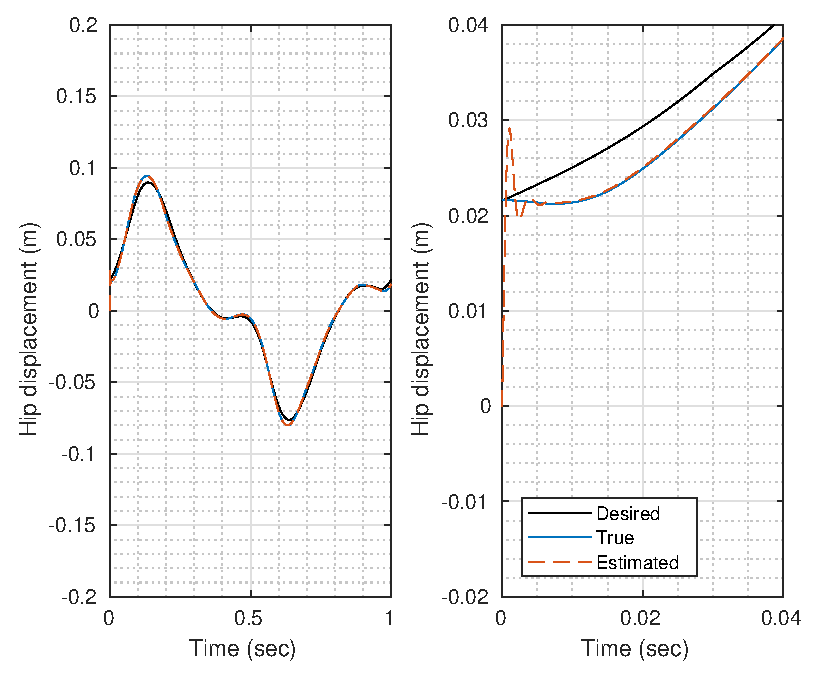
\includegraphics[width = \columnwidth]{Figs/q_hip_mu_1e-03.eps}
%	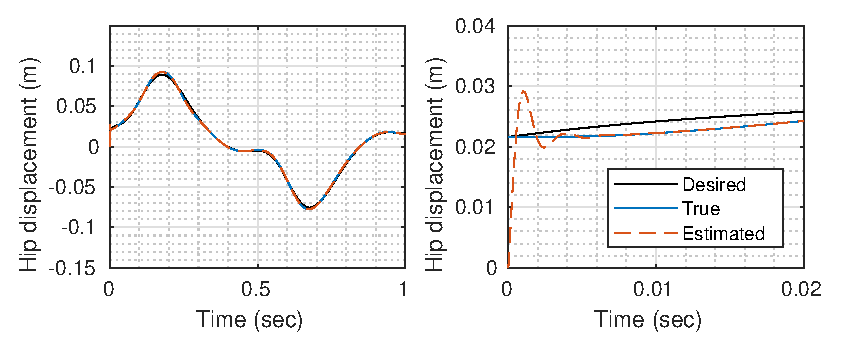
\includegraphics[width = \columnwidth]{Figs/q_hip_mu_fix_1e-03.eps}
%	\caption{ Simulation results from a desired hip movement, the controlled plant state and the estimated state. The right plot shows the signal in the first 20ms of simulation}
%	\label{fig:hip}
%	\end{center}
%\end{figure}
%
%
%\begin{figure}[h!]
%	\begin{center}
%	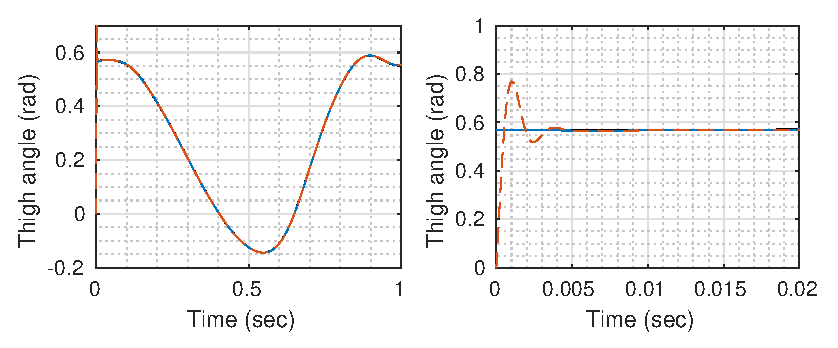
\includegraphics[width = \columnwidth]{Figs/q_thigh_mu_fix_1e-03.eps}
%	\caption{ Simulation results from a desired thigh movement, the controlled plant state and the estimated state from the HGO. The right plot shows the signal in the first 20ms of simulation}
%	\label{fig:thigh}
%	\end{center}
%\end{figure}
%
%
%\begin{figure}[h!]
%	\begin{center}
%	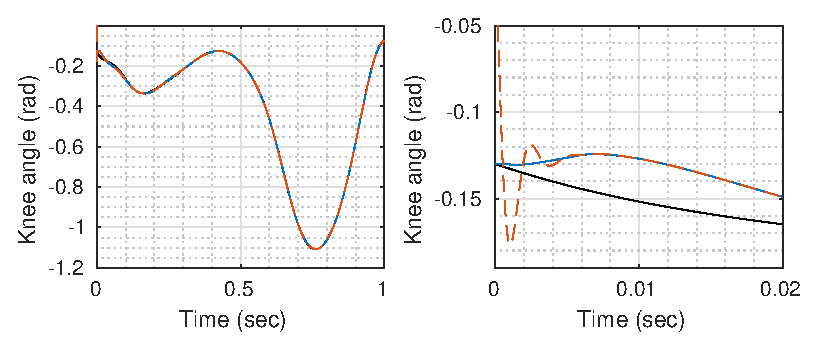
\includegraphics[width = \columnwidth]{Figs/q_knee_mu_fix_1e-03.eps}
%	\caption{ Simulation results from a desired knee movement, the controlled plant state and the estimated state. The right plot shows the signal in the first 20ms of simulation}
%	\label{fig:knee}
%	\end{center}
%\end{figure}
%
%
%\begin{figure}[h!]
%	\begin{center}
%	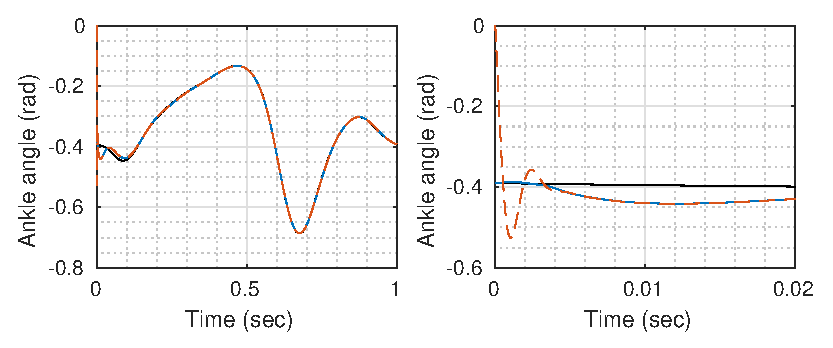
\includegraphics[width = \columnwidth]{Figs/q_ankle_mu_fix_1e-03.eps}
%	\caption{ Simulation results from a desired ankle movement, the controlled plant state and the estimated state. The right plot shows the signal in the first 20ms of simulation}
%	\label{fig:ankle}
%	\end{center}
%\end{figure}
%
%
% Velocity plots 
%
%
%\begin{figure}[h!]
%	\begin{center}
%	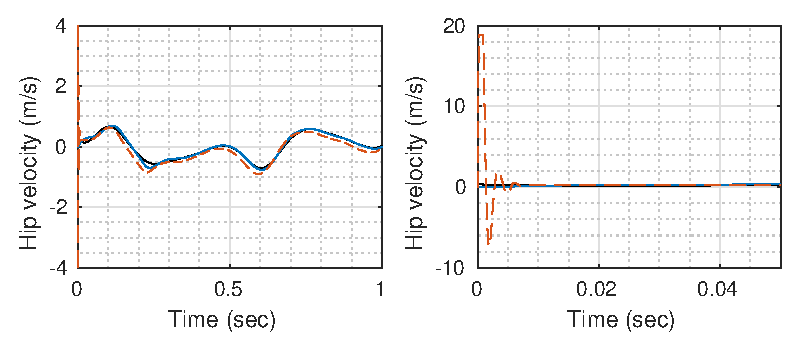
\includegraphics[width = \columnwidth]{Figs/dq_hip_mu_fix_1e-03.eps}
%	\caption{ Simulation results from a desired hip velocity, the controlled plant state and the estimated state. The right plot shows the signals behaviors until the first 50ms of simulation.}
%	\label{fig:dhip}
%	\end{center}
%\end{figure}
%
%
%\begin{figure}[h!]
%	\begin{center}
%	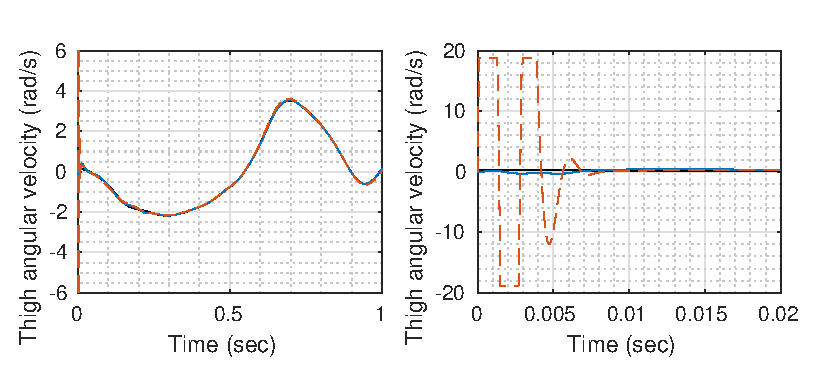
\includegraphics[width = \columnwidth]{Figs/dq_thigh_mu_fix_1e-03.eps}
%	\caption{Simulation results from a desired thigh velocity, the controlled plant state and the estimated state. The right plot shows the signal in the first 20ms of simulation.}
%	\label{fig:dthigh}
%	\end{center}
%\end{figure}
%
%
%\begin{figure}[h!]
%	\begin{center}
%	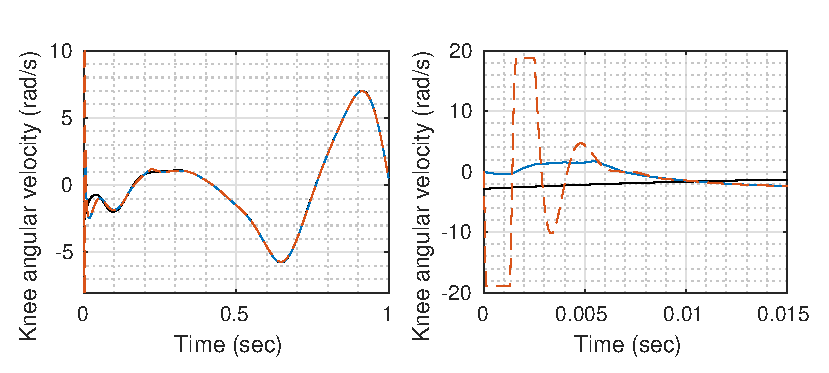
\includegraphics[width = \columnwidth]{Figs/dq_knee_mu_fix_1e-03.eps}
%	\caption{Simulation results from a desired knee velocity, the controlled plant state and the estimated state. The right plot shows the signal in the first 15ms of simulation.}
%	\label{fig:dknee}
%	\end{center}
%\end{figure}
%
%
%\begin{figure}[h!]
%	\begin{center}
%	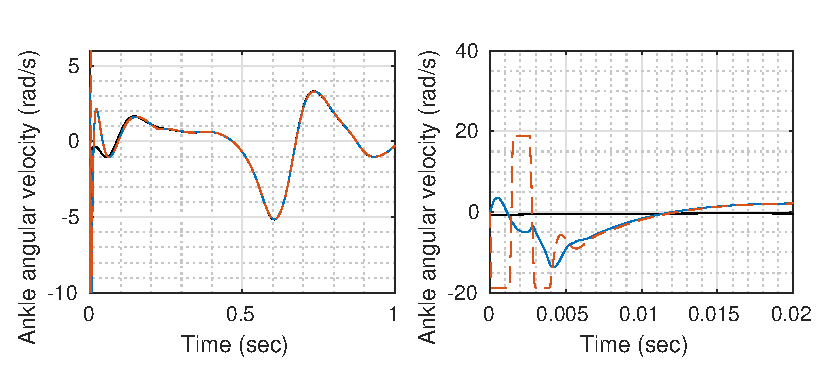
\includegraphics[width = \columnwidth]{Figs/dq_ankle_mu_fix_1e-03.eps}
%	\caption{Simulation results from a desired ankle velocity, the controlled plant state and the estimated state. The right plot shows the signal in the first 20ms of simulation.}
%	\label{fig:dankle}
%	\end{center}
%\end{figure}
%

\begin{table}[]
	\centering
	\caption{RMSE for HGO states and the desired trajectory in each joint of a prosthetic leg according to the observer gain $\mu$}
	\resizebox{\columnwidth}{!}{%
	\begin{tabular}{ccccccccc}
	\hline
	$\mu$      & $x_1$ (m) & $x_2$ (rad) & $x_3$ (rad) & $x_4$ (rad) & $\dot{x}_1$ (m/s) & $\dot{x}_2$ (rad/s) & $\dot{x}_3$ (rad/s) & $\dot{x}_4$ (rad/s) \\ \hline
	0.4e-3   & 0.0004 & 0.0002 & 0.0009  & 0.0004  & 0.0159  & 0.0117    &  0.0959   &  0.0492   \\
	1.9e-3   & 0.0035 & 0.0013 & 0.0033  & 0.0062  & 0.1120  & 0.0587    &  0.2405   &  0.6836   \\
	Variable & 0.0008 & 0.0004 & 0.0025  & 0.0059  & 0.0257  & 0.0375    &  0.2268   &  0.6640
	\end{tabular}
	\label{table:RMSE_track}
	}%
\end{table}

\begin{comment}
\begin{table}[]
	\centering
	\caption{RMSE of a human gait for each joint of a prosthetic leg with estimated states according to the observer gain $\mu$}
	\resizebox{\columnwidth}{!}{%
	\begin{tabular}{ccccccccc}
	\hline
	$\mu$      & $x_1$ (m) & $x_2$ (rad) & $x_3$ (rad) & $x_4$ (rad) & $\dot{x}_1$ (m/s) & $\dot{x}_2$ (rad/s) & $\dot{x}_3$ (rad/s) & $\dot{x}_4$ (rad/s) \\ \hline
	0.4e-3   & 0.0001 & 0.0036 & 0.0008  & 0.0024  & 0.2607  & 0.4228    &  0.3570   &  0.4065   \\
	1.9e-3   & 0.0004 & 0.0065 & 0.0015  & 0.0045  & 0.3973  & 0.7754    &  0.5952   &  0.8514   \\
	Variable & 0.0003 & 0.0065 & 0.0015  & 0.0045  & 0.3167  & 0.7724    &  0.5948   &  0.8512
	\end{tabular}
	\label{table:RMSE_est}
	}%
\end{table}
\end{comment}

A variable HGO gain adaptation is depicted in Fig.~\ref{fig:mu_comparison}. In Figs.~\ref{fig:SNR_comparison} and Fig.~\ref{fig:u_comparison} the same legend pattern in applied as in Fig.~\ref{fig:mu_comparison}, therefore blue, yellow and red represent $\mu_{1}$, $\mu_{2}$ and $\mu_{var}(t)$ respectively.

% --------------------TESTE ---------------
%
\begin{figure}[]
	\begin{center}
	\includegraphics[width = \columnwidth]{Figs/test.eps}
	\caption{Simulation results showing the adaptation from a variable $\mu$ converging to 0.001.}
	\label{fig:mu_comparison}
	\end{center}
\end{figure}
%
%
\begin{figure}[]
	\begin{center}
	\includegraphics[width = \columnwidth]{Figs/test.eps}
	\caption{Simulation results showing the adaptation from a variable $\mu$ converging to 0.001.}
	\label{fig:mu_comparison}
	\end{center}
\end{figure}
%

% -------------------------------------------

%
\begin{figure}[]
	\begin{center}
	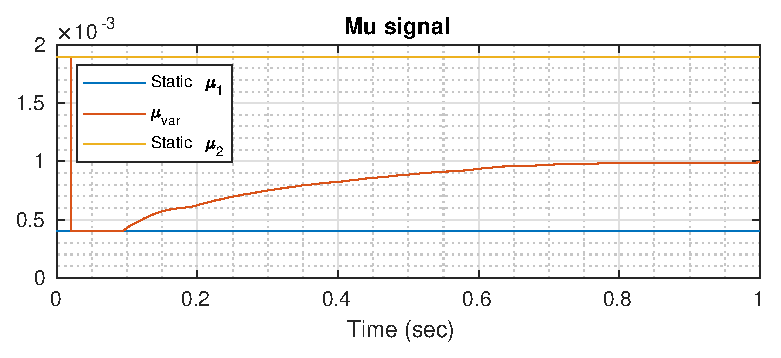
\includegraphics[width = \columnwidth]{Figs/mu_comparison.eps}
	\caption{Simulation results showing the adaptation from a variable $\mu$ converging to 0.001.}
	\label{fig:mu_comparison}
	\end{center}
\end{figure}
%
%
\begin{figure}[]
	\begin{center}
	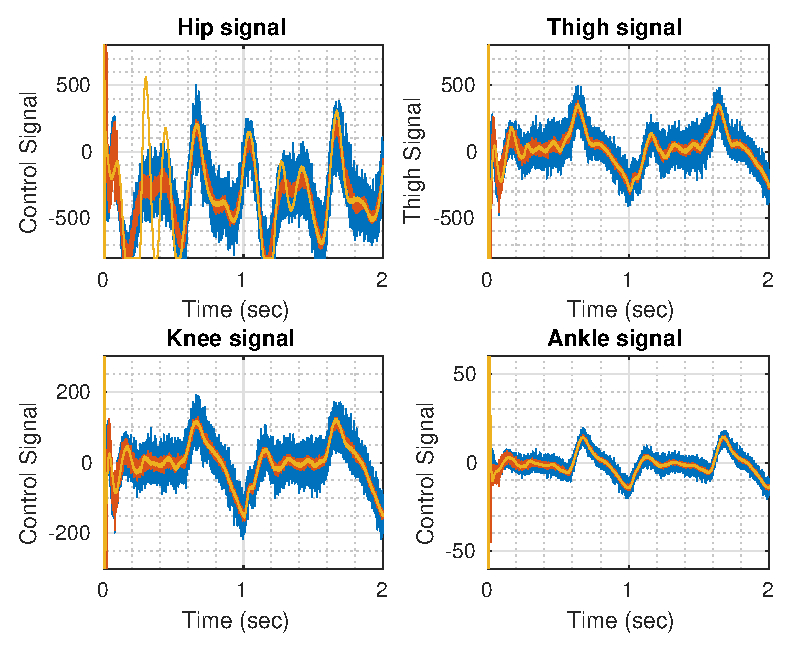
\includegraphics[width = \columnwidth]{Figs/u_comparison.eps}
	\caption{This graphic shows the difference between gain values and its filtering capacity. The control signal in blue represents the static gain $\mu = 0.0004$, which does not filter the noise as much as $\mu_{var}(t)$ in red or $\mu = 0.0019$ in yellow.}
	\label{fig:u_comparison}
	\end{center}
\end{figure}
%
%
\begin{figure}[]
	\begin{center}
	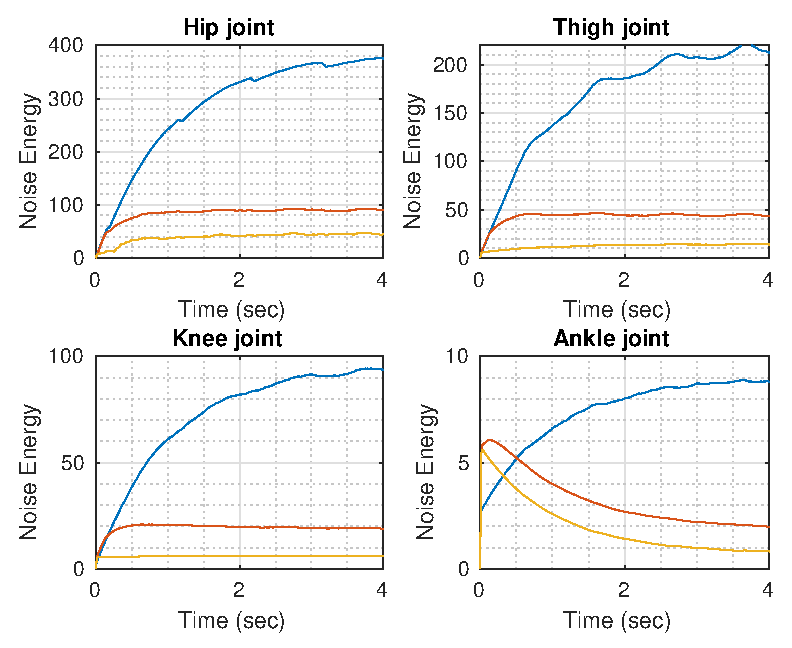
\includegraphics[width = \columnwidth]{Figs/SNR_comparison.eps}
	\caption{$\mu_{var}(t)$ in red is able to filter noise as good as $\mu = 0.0019$ in yellow.}
	\label{fig:SNR_comparison}
	\end{center}
\end{figure}
%
%
\begin{figure}[]
	\begin{center}
	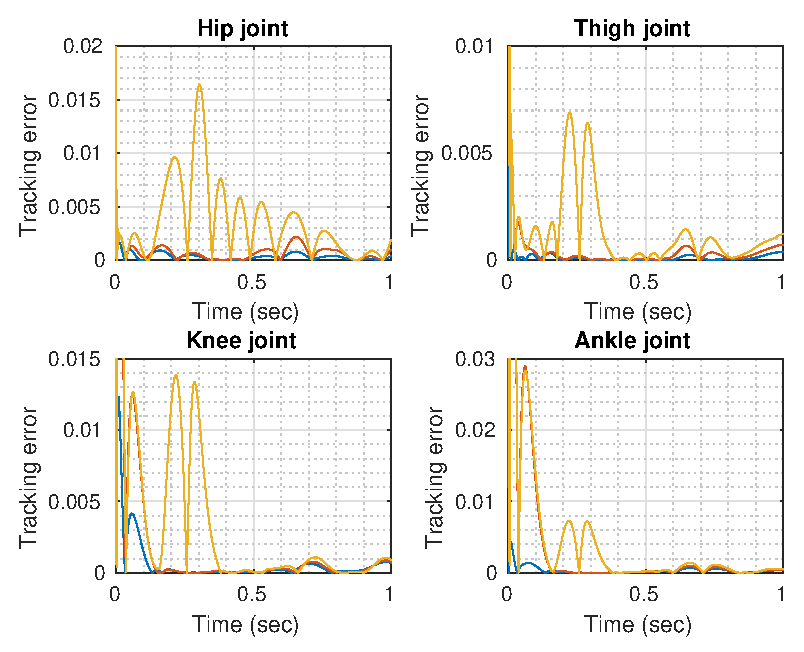
\includegraphics[width = \columnwidth]{Figs/q_error_comparison.eps}
	\caption{Using $\mu_{var}(t)$, in red, the system is able to track the trajectory as good as when $\mu = 0.0004$ in blue. For quantitative values, Table \ref{table:RMSE_track} shows tracking RMSE.}
	\label{fig:q_error_comparison}
	\end{center}
\end{figure}
%
By applying $\mu_{2}$, an apparent degradation in the closed-loop tracking error transient is shown in Table~\ref{table:RMSE_track} and Fig.~\ref{fig:q_error_comparison}. On the other hand, the noise amplitude in the control signal is acceptable as can be observed in Fig.~\ref{fig:u_comparison} with the corresponding measurement of the noise amplitude illustrated in Fig.~\ref{fig:SNR_comparison}. The noise amplitude was obtained by filtering the control input $u$ with a high-pass filter.
%

%
By reducing $\mu$ to the constant small value $\mu_{var}(t) = 0.0004$, the  tracking error transient is improved in exchange of an increase on the control signal noise, see  Fig.\ref{fig:SNR_comparison}, FIg.~\ref{fig:q_error_comparison} and Table~\ref{table:RMSE_track}.
%

%
On the other hand, when the time-varying $\mu_{var}(t)$ is implemented starting with the same large value for
$\mu_{var}(0) = 0.0019$, the tracking error transient is improved without reducing $\mu$ to a prohibitive value which can cause a large noise in the control signal. 
%

%
The time evolution of $\mu_{var}(t)$ is shown in Fig.\ref{fig:mu_comparison}, from which one can verify
that $\mu$ reaches a value of $\mu_{var}(t)=0.001$ depending on the noise power applied  to the system. 
This value is not known {\em a priori}. It is clear that care must be taken while reducing $\bar{\mu}$, since there exists a trade off between noise reduction and tracking accuracy.
%
%


%%%%%%%%%%%%%%%%%%%%%%%%%%%%%%%%%%%%%%%%%%%%%%%%%%%%%%%%%%%%%%%%%%%%%%%%%%%%%%%%
\section{Conclusions and Future Work}
\label{sec:Conclusions}
%\subsection{Conclusions}

In this paper we considered the state estimation problem of a robot/prosthesis control system with vertical hip displacement, thigh, knee and ankle joints.  It was verified that it is possible to apply HGO with dynamic gain in order to reduce the amount of noise in the control signal while assuring an reasonable output tracking error transient. Moreover, when a norm observer is available, domination techniques can be used to design the HGO dynamic gain to obtain global/semi-global practical tracking, via sliding mode control. An illustrative academic simulation example was presented.

Future possible topics of research are: (i) consider the full robot/prosthesis model including the ground reaction forces estimation; (ii) replace the conventional PID controller by a smooth version of the  output feedback sliding mode controller previous developed in \cite{POH:2011} in order  to increase the robustness of the closed loop system w.r.t. parameter uncertainties while assuring  global/semi-global stability properties and (iii) perform experimental results.

%%%%%%%%%%%%%%%%%%%%%%%%%%%%%%%%%%%%%%%%%%%%%%%%%%%%%%%%%%%%%%%%%%%%%%%%
\begin{footnotesize}
%%%
\bibliography{IEEEabrv,BibProtese,TVHGO} 
%
%\bibliographystyle{unsrt}
%\bibliography{BibProtese}
%

%
%%===============================================================
%%
%\appendix
%
%\subsection{Nominal Values}
%
%Plant nominal values can be taken into account to reduce conservatism in the HGO design. The plant could be rewritten as:
%%
%\begin{subequations}
%	\begin{eqnarray}
%		\dot{x}_1&=& x_2\,, \\
%		\dot{x}_2 &=& f(x_1,x_2,u,t) + \delta_f(x_1,x_2,u,t)\,, \quad u:=F_a\,,\\
%		y &=&  x_1\,,
%	\end{eqnarray}
%\end{subequations}
%%
%where the nominal part of the system dynamics is represented by
%%
%%
%\begin{eqnarray}
%f(x_1,x_2,u,t):=D_n^{-1}(x_1) u - D_n^{-1}(x_1) \left[ C_n(x_1,x_2) x_2+g_n(x_1)\right]\,, \nonumber
%\end{eqnarray}
%%
%while the uncertainties are concentrated in the term 
%%
%\begin{equation}
%	\begin{split}
%		\delta_f(x_1,x_2,u,t)\!\! := \!\!&\left[D^{-1}(x_1)-D_n^{-1}(x_1)\right]  u + \\
%		&\left[D_n^{-1}(x_1)C_n(x_1,x_2) - D^{-1}(x_1)C(x_1,x_2)\right] x_2 + \\
%		&\left[D_n^{-1}(x_1)g_n(x_1) - D^{-1}(x_1)g(x_1)\right]\,.
%	\end{split}
%\end{equation}
%%
%However, to simplify this presentation while keeping the main HGO design methodology, consider $C_n \equiv 0$, $g_n \equiv 0$ and, since $D$ is assumed known, we also have $D_n=D$.
\end{footnotesize}
%
\end{document}
%%%%%%%%%%%%%%%%%%% E N D  O F   F I L E %%%%%%%%%%%%%%%%%%%%%%%%%%%%%%%%%%


When the plant (\ref{eq:plantSS})--(\ref{eq:plantSaida}) admits a norm observer with $\omega$ defined in (\ref{eq:xboundfromw}) such that 
%
\begin{equation}
|x(t)| \leq \bar{\varphi}_o(\omega(t),t) + \pi_o(t)\,,\label{eq:xboundfromw1}
\end{equation}
%
then the signal $\nu$ satisfies (see \cite{POH:2011} for details):
%
\begin{equation}
|\nu| \leq \psi_\nu(\omega,t)+\pi_3\,,\label{eq:boundonnu}
\end{equation}
%
for some non-negative function $\psi_\omega$ and vanishing term $\pi_3$ depending on  initial conditions.  Moreover, the signal $\omega$ is such that the following inequality holds (see \cite{POH:2011} for details):
%
\begin{equation}\label{eq:boundonomegadot}
\left|\dot{\omega}\right| \leq \psi_\omega(\omega,t)+\pi_1\,,
\end{equation}
%
respectively, for some non-negative functions $\psi_\omega$  and vanishing terms $\pi_1$ depending on  initial conditions. 
%
In order to obtain a norm bound for the time derivative of $\mu$
(\ref{eq:def_mu}) we calculate $\dot{\mu}$ by the expression:
%
\begin{equation}
\dot{\mu}(t)\!=\!-\frac{\mu^2}{\bar{\mu}} \left[\frac{\partial
\psi_\mu}{\partial \omega} \dot{\omega}+\frac{\partial
\psi_\mu}{\partial t}\right]\,. \label{eq:def_mudot2}
\end{equation}
%
Note that, $\dot{\mu}$ is a piecewise continuous time signal which
can be upperbounded by
%
\begin{equation}
|\dot{\mu}(t)|\!\leq\!\frac{\left|\frac{\partial
\psi_\mu}{\partial \omega}\right|}{1+\psi_\mu} \mu
|\dot{\omega}|+\frac{\left|\frac{\partial \psi_\mu}{\partial
t}\right|}{1+\psi_\mu}\mu\,. \label{eq:mudotbound}
\end{equation}
%
Hence, one has that:
%
\begin{equation}
\mu|\nu| \leq
\frac{\psi_\nu}{1+\psi_\mu}\bar{\mu}+\mu\pi_3\,,\label{eq:boundonmunu}
\end{equation}
%
and
%
\begin{equation}
\mu|\dot{\omega}| \leq
\frac{\psi_\omega}{1+\psi_\mu}\bar{\mu}+\mu\pi_1\,.\label{eq:boundonmudotomega}
\end{equation}
%
Now, choose the adapting function $\psi_\mu$ in
(\ref{eq:def_mu}) so that the following property holds with
$\psi_\nu$ in (\ref{eq:boundonnu}) and $\psi_\omega$ in
(\ref{eq:boundonomegadot}):

\medskip
%
\begin{description}
\item[(P0)] $\psi_\nu\,, \
\psi_\omega \leq c_{\mu 0}(1+\psi_\mu)$, $\forall t \in [0,t_M)$,
where $c_{\mu 0}\geq 0$ is a {\em known} constant.
\end{description}
%
\medskip

If  $\psi_\mu$ satisfies (P0) then, from (\ref{eq:boundonmunu})
and (\ref{eq:boundonmudotomega}), $\mu|\nu|$ and
$\mu|\dot{\omega}|$ can be bounded by
%
\begin{align}
\mu|\nu| &\leq
\mathcal{O}(\bar{\mu})+\mu\pi_3\,.\label{eq:boundonmunu1}\\
\mu|\dot{\omega}| &\leq
\mathcal{O}(\bar{\mu})+\mu\pi_1\,.\label{eq:boundonmudotomega1}
\end{align}
%
Moreover, our strategy is to design $\psi_\mu(\omega,t)$ such that the
following  property holds:

\medskip
%
\begin{description}
\item[(P1)] $\left|\frac{\partial \psi_\mu}{\partial
\omega}\right|\,, \ \left|\frac{\partial \psi_\mu}{\partial
t}\right|\leq c_{\mu 1}(1+\psi_\mu)$, $\forall t \in [0,t_M)$, where
$c_{\mu 1}\geq 0$ is a {\em known} constant.
\end{description}
%
\medskip

This property is trivially satisfied by polynomial $\psi_\mu$ with
positive coefficients. Now, with $\psi_\mu$ satisfying (P1), one has that:
%
\begin{equation}
|\dot{\mu}(t)|\!\leq\!c_{\mu 1} \mu |\dot{\omega}|+c_{\mu 1}
\mu\,. \label{eq:mudotbound1}
\end{equation}
%
Therefore, from (\ref{eq:mudotbound1}), (\ref{eq:boundonmunu1})
and (\ref{eq:boundonmudotomega1}) the following holds:
%
\begin{equation}
|\dot{\mu}(t)|\,, \ \mu|\nu| \leq \mathcal{O}(\bar{\mu}) + \mu
\pi_4\,, \label{eq:mudotandmunu1}
\end{equation}
%
where $\pi_4:=c_{\mu 1} \pi_1 +\pi_3$.

Finally, if $\psi_\mu$ is designed so that (P0)--(P1) hold and {\em finite escape is avoided}\footnote{This can be guaranteed if an additional technical Property is satisfied, see \cite{POH:2011} for details. Here, we omitted this property just to simplify the paper presentation.}, then
from (\ref{eq:mudotandmunu1})  one can verify
that there exists a finite $t_\mu \in [0,t_M)$ such that:
%
\begin{equation}
|\dot{\mu}(t)|\,, \ \mu |\nu| \leq \mathcal{O}(\bar{\mu})\,, \quad
\forall t \in [t_\mu,t_M)\,. \label{eq:mudotmunu1}
\end{equation}
%
In this case, the stability and/or convergence analysis  can be carried out by noting that the output tracking error dynamics (and the full error system dynamics) is ISS w.r.t. HGO estimate error $\tilde{x}$ which is of order $\mathcal{O}(\bar{\mu})$ after the small finite time instant $t_\mu$.

